\documentclass[10pt, twocolumn]{article}
\author{Daniel Cowgill and Graham Lowe}
\usepackage[pdftex]{color,graphicx}
\title{juice}

\begin{document}

\maketitle

\section{User Interface Framework}

\subsection{Background}

In 2004, Community Connect Inc. started a project to rewrite their
entire code-base. We finished this initiative in late 2007. The
end-result was a software architecture that facilitated concurrent
development of the database and domain logic layers of their
application. Despite productivity gains in the \emph{backend}
layers of the system, \emph{frontend} (i.e., user interface)
development was still arduous.

\subsection{Problem}

To help you understand the deficiencies that existed with user
interface development, we will describe the typical workflow for
developing a new interface. But first we will introduce the roles
involved in the workflow\footnote{we've omitted roles (e.g.,
  project manager) that are non-essential to understanding the
  workflow problem.}:

\begin{itemize}
\item The \emph{product designer} specifies initial requirements
  for a product.
\item The \emph{interaction designer} translates initial
  requirements to user interface requirements, often expressing
  them as wireframes (i.e., a low-fidelity paper-based graphical
  specification for the product).
\item The \emph{frontend developer} interprets user interface
  requirements from wireframes, creating a non-functional HTML
  user interface prototype.
\item The \emph{backend developer} interprets requirements,
  creating a database model and writing domain logic code to
  implement the product's functionality; she also integrates this
  \emph{backend} with the HTML user interface prototype, resulting
  in a functional product.
\item The \emph{quality assurance specialist} tests the functional
  product, ensuring that it is consistent with the product
  specification.
\end{itemize}

Now that we are familiar with the roles, we'll describe a typical
workflow for developing a user interface; this workflow is
depicted in Figure \ref{workflow}.

\begin{figure*}
  \centering
  \includegraphics[scale=0.50]{workflow.png}
  \caption{Inefficient UI development workflow}
  \label{workflow}
\end{figure*}

The product designer creates rudimentary requirements for a
product and hands them off to the interaction designer. He uses
these requirements to create wireframes, which he then gives to a
frontend developer who uses a proprietary user interface
prototyping tool to generate an HTML-based prototype. The frontend
developer disseminates this generated HTML to the backend
developer who is responsible for integrating this HTML with
PHP\cite{PHP} code to create a functional product. Once the
product is functional, it is ready for inspection by the quality
assurance specialist. If the QA specialist finds user interface
defects, the issue will be sent to the frontend developer who then
revises the HTML, which must then be reintegrated by the backend
developer. This cycle repeats until the product is deemed perfect.

There are several issues with the workflow we've described. The
frontend developer wastes time creating an HTML prototype of the
user interface. Once created, the prototype serves as a
specification of the product's HTML, so subsequent modifications
to the HTML must first be made by the frontend developer to the
prototype and then translated to the functional product by the
backend developer. It would be better if there was a single
version of the HTML, preferably in the end product. Another
deficiency is that the QA specialist must wait for the backend
developer to finish his work before she can identify problems that
are only apparent when working with a functioning product.
Furthermore, correcting these defects often result in changes to
the data model and domain logic code, so that in addition to any
HTML reintegration, the backend developer will have to make
changes to the backend layer as well. If the QA specialist could
test the functional product earlier in the process, then less
rework would be required. Another issue with the process is that
frontend developers use a high-level language to describe the user
interface, treating HTML as a low-level target language. Backend
developers must deal with this generated HTML---this HTML is not
designed for human comprehension---making integration with PHP
code more difficult.

It also worth mentioning that because of the sequential nature of
this workflow, it is futile to add frontend development resources
without adding backend development resources and vice-versa. An
improved workflow would allow concurrent frontend and backend
development.

\subsection{Towards a Solution}

Before designing the user interface framework, we first analyzed
the issues with workflow and determined that many of the problems
could be alleviated by enforcing a clear separation between the
\emph{frontend} and \emph{backend} development tasks. Given this
prerequisite, we set about defining other essential requirements
for the framework. To save the wasted time of creating prototypes
and to allow the product designer and QA specialist to provide
feedback earlier in the workflow process, we determined that the
framework should be able to produce working user interfaces
without a functional backend. We also liked the idea of using a
high-level user interface description language. Also, with the
popularity of smart interfaces like Gmail \cite{gmail}, we added
the requirement that the framework should have good support for
AJAX.

With these initial set of requirements, we started thinking about
software engineering issues. It was important that the framework
allow the creation of arbitrarily complex user interfaces while
ensuring that the code to do so wasn't overly complex; to achieve
this goal, we decided that the framework should allow interfaces
to be built by combining several simple components into a single
component.

\subsection{Prototyping}

Armed with these requirements, we decided that we needed to
prototype some solutions to gain familiarity with the technical
challenges.

We wrote our first framework prototype in PHP. This version of the
framework required the client programmer to specify the user
interface as a series of PHP objects which map to generated HTML
and JavaScript. Some of the benefits of using PHP were:

\begin{itemize}
\item Backend programmers were already familiar with language.
\item PHP, because it was initially designed as a templating
  language, allows HTML to be easily generated.
\end{itemize}

However, we also found some drawbacks:

\begin{itemize}
\item The programming model was very complex because PHP code is
  executed in the server and JavaScript code is executed in the
  browser.
\item Because the backend code was also written in PHP, using PHP
  as a frontend language invites bleed through of non-user
  interface code to user interface code and vice-versa.
\end{itemize}

We soon realized that PHP wasn't a good fit for the framework, so
we decided to write our second prototype in pure JavaScript. Some
of the upfront benefits were:

\begin{itemize}
\item Frontend programmers are familiar with language.
\item JavaScript is arguably a more powerful language than PHP.
\item AJAX support is built into the language.
\item Enforces a clear separation of concerns because the frontend
  is written in a different language than the backend.
\end{itemize}

Here were some of the drawbacks:

\begin{enumerate}
\item JavaScript, or rather browser implementations of JavaScript,
  are notorious for being quirky.
\item Although some of the programmers were familiar with
  JavaScript, the sophistication of the framework would require
  deeper knowledge.
\end{enumerate}

After prototyping, we found ourselves enamored with JavaScript.
Although it is much maligned, at its core it's a great language.
We found its combination of first class function, closures, and
uniform syntax to be very powerful. Furthermore, we found that
there are several open source libraries that hide the need to
write special workaround code for browser quirks.

\subsection{juice}

Once we had finished prototyping, we set out to work on our
framework in earnest. In this section, we describe the result of
our efforts---a framework we called \emph{juice}, which stands for
\textbf{J}avaScript \textbf{U}ser \textbf{I}nterface
\textbf{C}ompiled \textbf{E}nvironment.

Some qualitative goals we tried to achieve when creating juice
were: making it as declarative as possible, keeping the core
concise, minimizing complexity, and ensuring its components were
orthogonal.

While juice is a framework, it can also be thought of as a
language for describing a user interface, so we'll explain it as
such---by enumerating its primitives and means of composition.
Figure \ref{architecture} illustrates juice's architecture.
\begin{figure}
  \centering
  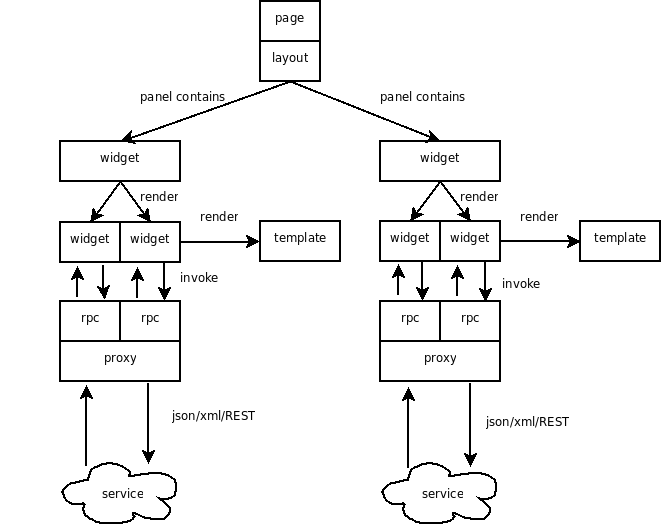
\includegraphics[scale=0.35]{architecture.png}
  \caption{juice}
  \label{architecture}
\end{figure}

\subsubsection{Primitives}
\begin{itemize}
\item A \emph{RPC} represents a remote service that is implemented
  by the backend. RPC definitions are written by a backend
  programmer and specify the expected input and output values for
  an RPC function call. RPC definitions are fully declarative.
  Here's an example RPC definition:
\begin{verbatim}
juice.rpc.define(
  {name: 'add_bulletin',
   service_name: 'add_bulletin',
   req_spec: {subject: 'string',
              body: 'string'},
   rsp_spec: null});
\end{verbatim}

  RPCs are invoked by widgets. Because of their asynchronous
  nature, the caller must supply a callback function which is
  passed the response from the backend service. Here's an example
  of how to call an RPC:

\begin{verbatim}
proj.bulletins.add_bulletin(
  {subject: "Lunch",
   body: "Free lunch for everybody!"},
  function(rsp) {
     // Do something with response
     ...
  });
\end{verbatim}

  Each RPC invocation is handled by a proxy. This layer of
  indirection can provide several benefits. For example, a proxy
  can package several RPCs into a single network request, reducing
  the number of network round-trips. Or a mocking proxy may be
  used to fake a backend service, allowing the user interface to
  be almost completely functional before the backend service is
  even implemented. In either case, the proxy behavior is
  completely transparent to the caller of the RPC.

\item \emph{Widgets} describe user interface behavior and
  presentation. Widgets can call RPCs to retrieve or manipulate
  data. A widget's presentation is specified via its template.

  Here's an example widget definition:
\begin{verbatim}
juice.widget.define(
  'username_and_photo',
  function(that, my, spec) {
    var info = {
      username: spec.username,
      username_url:
        proj.pages.user.url(spec),
      image_url: spec.image_url
    };

    my.render =
      templates.user_and_photo(info);
    });
\end{verbatim}

\item A \emph{template} defines a widget's HTML presentation
  through a custom templating language that is compiled down to a
  JavaScript function that is optimized for rendering speed.

  Here's an example template:
\begin{verbatim}
<form disabled="disabled">
  
  <legend>{{label}}</legend>
  
  
  {{input}}
  
  
  {{button}}
  
</form>
\end{verbatim}
\end{itemize}

\subsubsection{Means of Composition}
\begin{itemize}
\item \emph{Widgets} can be composed from other widgets. This
  feature allows client programmer to create widgets of arbitrary
  complexity through composition while keeping the code as simple
  as possible.

  Here's an example of a composite widget (composed from 5 smaller
  widgets):
\begin{verbatim}
juice.widget.define(
  'my_form',
  function(that, my) {
    var form =
      proj.widgets.form({submit_label: 'search'})
       .add('gender',
            proj.widgets.gender())
       .add('orientation',
            proj.widgets.orientation())
       .add('age_range',
            proj.widgets.age_range_input())
       .add('extra', w.extra());

    my.subscribe(
      form, 'submit',
      function(data) {
        juice.log(juice.dump(data));
      });

    my.render = form.render;

    form.init();
  });
\end{verbatim}


\item A \emph{page} definition specifies how a set of widgets are
  to be placed on a web-page using a layout definition.

A layout specifies the panels that appear on page. Here's an
example of a layout definition that defines a top panel, two
middle panels, and a bottom panel:
\begin{verbatim}
juice.layout.define(
  'two_column',
  {top: null,
   middle_: {middle_left: null,
             container_:
               {middle_right: null}},
   bottom: null});
\end{verbatim}

And here's an example page definition:
\begin{verbatim}
juice.page.define(
  {name: 'bulletins',
   title: 'Bulletins',
   path: '/bulletins/',
   layout: proj.layouts.two_column,
   widget_packages:
     ['bulletins', 'message_center'],
   init_widgets: function(args) {
     return {
       top: [
         w.core.login_assertion(),
         w.core.global_nav()],
       middle_left:
         [w.message_center.nav()],
       middle_right:
         [w.bulletins.uber_inbox()]};
   }
  });
\end{verbatim}
\end{itemize}

\subsubsection{Packaging and Compilation}

To support large-scale software development, juice requires
organizing widgets and RPCs into packages. Packages allow the
client programmer to define widgets and utility functions that are
hidden. Juice also requires a compilation step to create a
functional user interface. During this build step, the following
tasks are performed:

\begin{itemize}
\item Source code is checked for syntax errors and software
  engineering errors (e.g., cyclical dependencies).
\item Juice programming constructs are compiled into appropriate
  JavaScript functions and HTML. For example, templates are
  compiled into JavaScript functions that are optimized for
  rendering performance and page definitions are compiled into
  a corresponding HTML representation.
\item RPC and widget packages are compiled into source files that
  are scoped such that local function and widget definitions are
  hidden. Also, dependency information is extracted so that the
  resulting HTML pages include a minimal amount of external
  JavaScript files.
\item JavaScript is optimized into its most compact representation
  to reduce the amount of bandwidth required to deliver a file.
\end{itemize}

\subsection{Improved Workflow}

Juice provides a clear separation between frontend and backend
development tasks and the ability to \emph{mock} backend services
to create a standalone functional user interface. This allows us
to define an improved workflow which is illustrated in Figure
\ref{improved-workflow}.
\begin{figure*}
  \centering
  \includegraphics[scale=0.50]{improved_workflow.png}
  \caption{Improved UI development workflow}
  \label{improved-workflow}
\end{figure*}

In this workflow model, changes to the user interface don't
require a integration work by the backend developer. Not only does
this remove a serial step in the original workflow, but it allows
backend and frontend resources to be added to a project
independently. Furthermore, because a functional user interface
can be produced for a product without a functional backend, user
interfaces can be tested before the backend is completed. Another
benefit of this approach is that it allows multiple experimental
user interfaces to use the same backend services.

\subsection{Status}

While the juice framework is complete\footnote{We still have to
  write end-user documentation.}, it has yet to be used in
Community Connect Inc's production user interface code. This
daunting task has been planned for my Spring semester internship.

The core of the juice framework is approximately 4,200 lines of
JavaScript (including whitespace and comments), 300 lines of
Python, and 50 lines of the custom template language. We also
produced a juice demo application, a product similar to Google's
Gmail. This application consists of approximately 3,250 lines of
JavaScript and 1,050 lines of the custom template language.

\begin{thebibliography}{99}

\bibitem{PHP} http://www.php.net/

\bibitem{gmail} http://www.gmail.com/

\end{thebibliography}

\end{document}
